\chapter{METODOLOGI}

% Ubah konten-konten berikut sesuai dengan isi dari metodologi

\section{Data dan Peralatan}

\textbf{Data}
\begin{enumerate}
    \item Input Toucpad
\end{enumerate}

\textbf{Peralatan}
\begin{enumerate}
    \item Laptop Asus Zenbook 13
    \item Touchpad Wireless 
    \item Kursi Roda Elektrik
    \item Raspberry Pi 4
\end{enumerate}

\section{Metode yang digunakan}
% Dahului dengan gambar Blok Diagram, kemudian pada bagian berikutnya jelaskan masing- masing blok.
% Contoh input gambar dengan format *.jpg
\begin{figure} [H] \centering
  % Nama dari file gambar yang diinputkan
  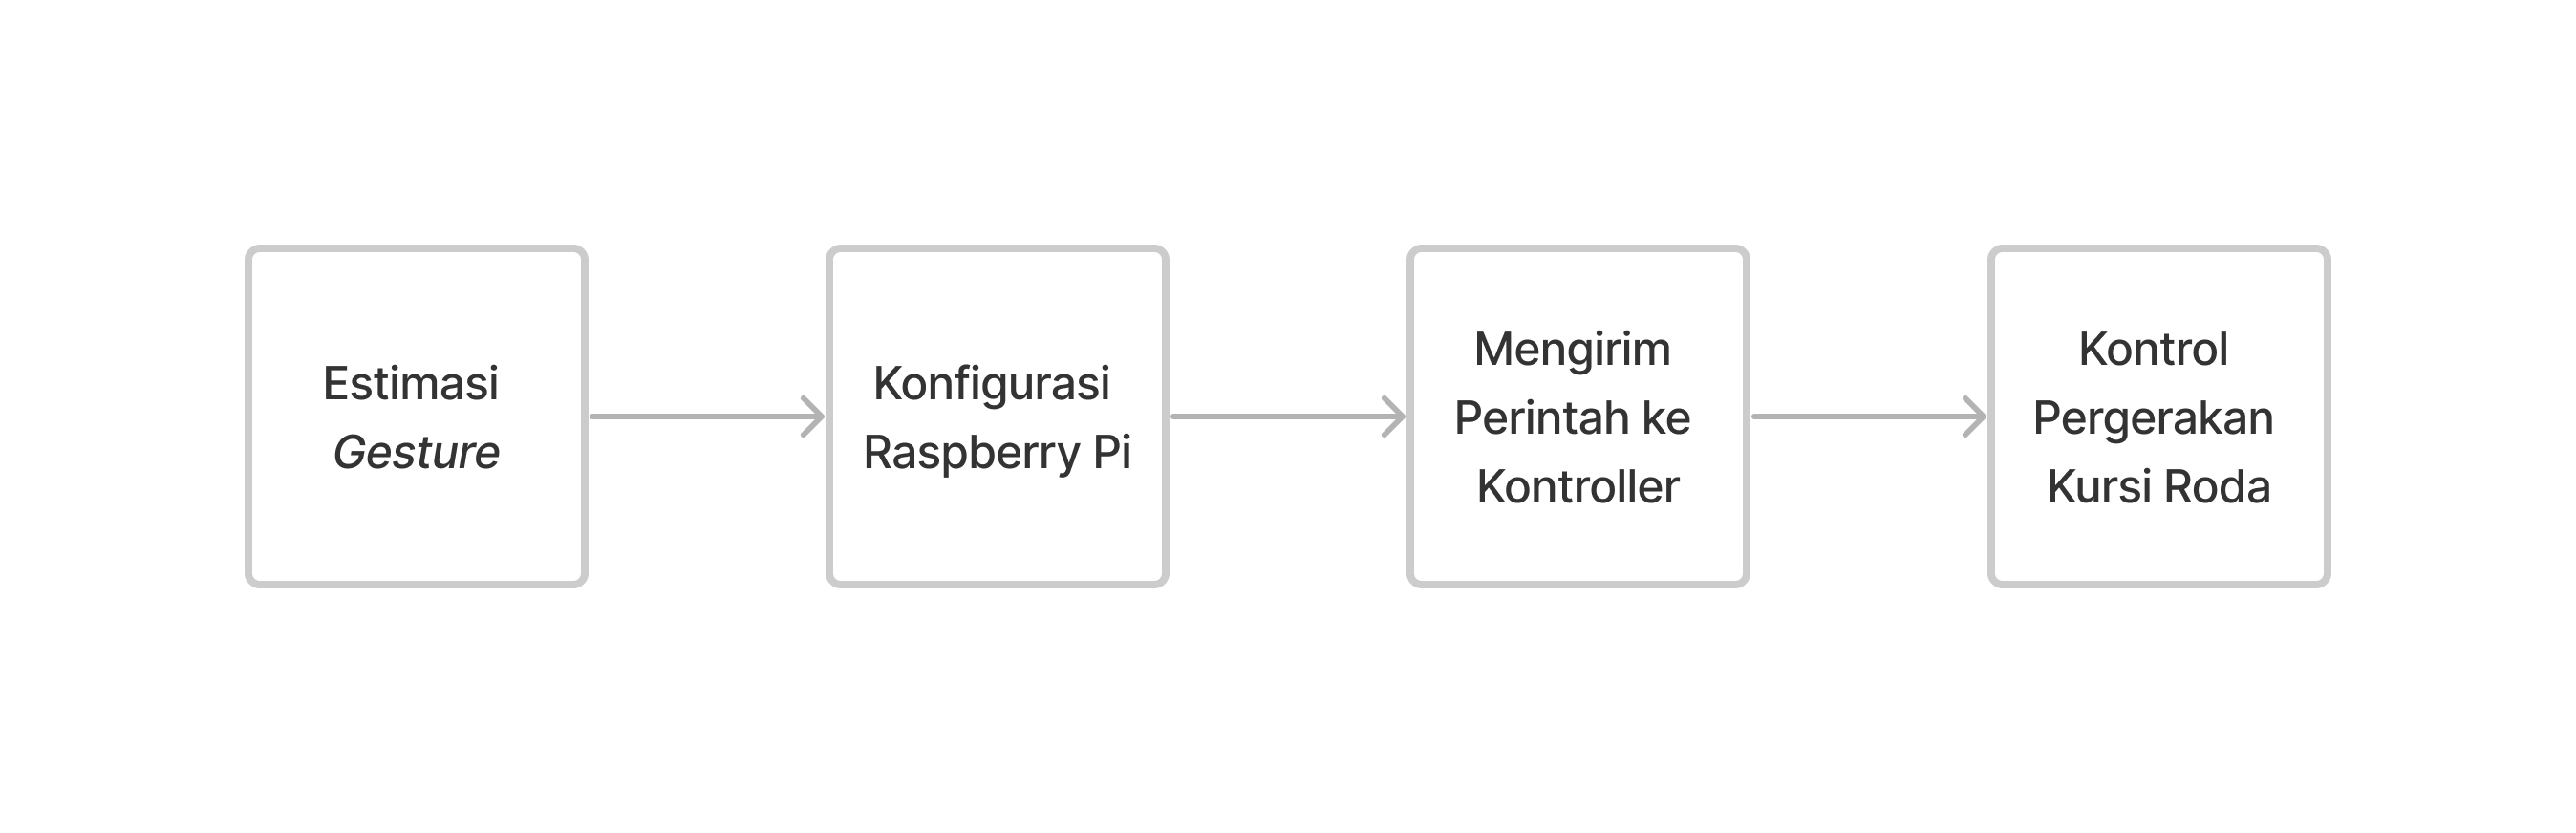
\includegraphics[scale=0.3]{gambar/metodologi.jpg}
  % Keterangan gambar yang diinputkan
  \caption{Metodelogi}
  % Label referensi dari gambar yang diinputkan
  \label{fig:metodelogi}
\end{figure}

% Contoh penggunaan referensi dari gambar yang diinputkan
\subsection{Estimasi Gesture}
Pada bagian ini saya menggunakan touchpad untuk menerima gesture. Saat jari memberikan gesture maka touchpad akan langsung mengestimasi gerakan apa yang diberikan oleh jari. setelah touchpad tau gerakan apa yang diberikan, output akan dikirimkan kepada Raspberry pi untuk diklasifikasi.

\subsection{Konfigurasi Raspberry Pi}
Disini saya memilih untuk menggunakan Raspberry Pi sebagai kepala dari rangkaian penelitian ini. pada raspberry pi dilakukan konfigurasi agar dapat mengklasifikasikan gesture apa yang diberikan oleh touchpad. Setelah dilakukan konfigurasi berdasarkan tiap-tiap gesture, maka akan dikirim data kepada kontroller

\subsection{Kontrol Pergerakan Kursi Roda}
Setelah kontroller menerima data dari raspberry pi, data tersebut langsung di jalankan sehingga kursi roda akan bergerak berdasarkan data yang telah diklasifikasikan oleh raspberry pi

% Pada \emph Blok Diagram \ref{fig:metodelogi}. Dapat dilihat bahwa pertama adalah mengestimasi gesture yang diberikan kepada touchpad. Setelah diestimasi maka raspberry pi akan melakukan konfigurasi dari gesture yang diberikan. setelah itu raspberry pi akan mengirimkan perintah ke kontroller karena gesture sudah di terkonfigurasi. kursi roda akan bergerak sesuai dengan perintah yang dikirim oleh raspberry pi

